% -----------------------------------------------
% Template for ISMIR Papers
% 2016 version, based on previous ISMIR templates

% Requirements :
% * 6+1 page length maximum
% * 2MB maximum file size
% * Copyright note must appear in the bottom left corner of first page
% (see conference website for additional details)
% -----------------------------------------------

\documentclass{article}
\usepackage{ismir,amsmath,cite}
\usepackage{graphicx}
\usepackage{color}
\usepackage{microtype}


% Title.
% ------
\title{A Dataset \& Approach for Automatic Practice Logging}

% Note: Please do NOT use \thanks or a \footnote in any of the author markup

% Single address
% To use with only one author or several with the same address
% ---------------
\oneauthor
{R. Michael Winters}
{Georgia Tech Center for Music Technology\\Georgia Institute of Technology, Atlanta GA}

% Two addresses
% --------------
%\twoauthors
%  {First author} {School \\ Department}
%  {ond author} {Company \\ Address}

%% To make customize author list in Creative Common license, uncomment and customize the next line
%  \def\authorname{First Author, Second Author} 


% Three addresses
% --------------
%\threeauthors
%  {First Author} {Affiliation1 \\ {\tt author1@ismir.edu}}
%  {Second Author} {\bf Retain these fake authors in\\\bf submission to preserve the formatting}
%  {Third Author} {Affiliation3 \\ {\tt author3@ismir.edu}}

%% To make customize author list in Creative Common license, uncomment and customize the next line
%  \def\authorname{First Author, Second Author, Third Author} 

% Four or more addresses
% OR alternative format for large number of co-authors
% ------------
%\multauthor
%{First author$^1$ \hspace{1cm} Second author$^1$ \hspace{1cm} Third author$^2$} { \bfseries{Fourth author$^3$ \hspace{1cm} Fifth author$^2$ \hspace{1cm} Sixth author$^1$}\\
%  $^1$ Department of Computer Science, University , Country\\
%$^2$ International Laboratories, City, Country\\
%$^3$  Company, Address\\
%{\tt\small CorrespondenceAuthor@ismir.edu, PossibleOtherAuthor@ismir.edu}
%}
%\def\authorname{First author, Second author, Third author, Fourth author, Fifth author, Sixth author}


\sloppy % please retain sloppy command for improved formatting

\begin{document}

%
\maketitle
%
\begin{abstract}
Musicians spend countless hours practicing their instruments.  To document, share, and organize this time, musicians commonly use practice charts to log the quantity and content of their practice. However, manual techniques require time, dedication, and experience to master, are prone to fallacy and omission, and ultimately can not capture many of the subtle nuances involved.  This paper presents an interesting alternative: by analyzing and classifying the audio produced while practicing, logging can occur automatically, with levels of detail, accuracy, and ease that would not be possible otherwise. Towards this goal, we introduce the problem of Automatic Practice Logging (APL), including a discussion of the benefits and unique challenges it raises. We then describe a new dataset of over 600 annotated recordings of solo piano practice, which can be used design and evaluate APL systems. After framing our approach to the problem, we present an algorithm designed to align short segments of practice audio with reference recordings using pitch chroma, and dynamic time warping.

% There are many benefits to tracking and logging practice done with musical instruments.  Traditional techniques use paper and pencil to record the content, quantity and quality of practice. In this paper, we propose a method to enable this process to occur automatically, with greater precision and ease than manual techniques. After providing additional motivation and context for automatic practice logging (APL), we describe its unique challenges. We then introduce an approach for labeling practice tracks using a form of audio-to-audio matching. Using a subset of 7 hours of practice, 128 tracks, and three pieces, our algorithm performs with $76.6\%$ accuracy.
\end{abstract}
%
\section{Introduction}\label{sec:introduction}

Musicians spend hundreds if not thousands of hours practicing their instruments. 
%Practice occurs in many contexts, sound environments, and with many different instruments. 
While a musical performance might occur in linear-time and with few note-errors, practice is characterized by repetitions, pauses, mistakes, various tempi, and fragmentation.
It can also take a variety of forms, including technique exercises, improvisation, repertoire work, and sight-reading. It can occur with any musical instrument (often with many simultaneously), and can take place in a range of acoustic environments.    

Within this context, we present the problem of automatic practice logging (APL), which attempts to identify and characterize the content of musical practice from recorded audio \textit{in situ}.  By its nature, an APL system must be robust to wrong notes, pauses, repetitions, fragmentation, dynamic tempi, and all of the other ``errors" of practice. It should be able to operate in challenging acoustic environments, work with any instrument, and even with many simultaneously. Most importantly, it needs to identify \textit{what} is being practiced and what \textit{type} of practice is occurring, so that it can describe and transcribe its content.    

%These attributes present only a few of the challenges to automatically identifying and characterizing the content of practice.
%Changed "classification" to "identification"{\color{red}{reader will not understand context of classification here}}

Despite these challenges, the landscape for automatic practice logging (APL) is rich and could be of high-impact to musicians at all levels. As compared to manual techniques, an APL system can offer unprecedented levels of detail, ease, and accuracy, not to mention additional advantages of digitization. The output of an APL system could help performers engage in smarter, more efficient practice, provide educators with more detailed accounts of practice, and as part of an intelligent mobile computing application, could serve as a practice companion. For the field of Music Information Retrieval (MIR), practice offers an interesting and challenging area of application. Considering the many thousands of musicians practicing a diversity of instruments on an almost daily basis, the amount of audio from recorded practice could easily surpass that of performance and studio recordings, offering a wide space for future work. 

%classification process {\color{red}{You really have to stop talking about classification without saying what is being classified in what categories. Why don't you properly define the task before talkinga bout the challenges?}} more difficult than other music classification tasks.  
%The system must be able to recognize the piece that is being played even for short excerpts, and must be robust to wrong notes, widely varying tempi, fragmentation, sporadic jumps within a piece, and also recognize when a piece has changed completely. 

%Despite these challenges, the potential rewards of an APL system are many, and have high-impact for practicing musicians at all skill levels. {\color{red}{Didn't you already start the second to last paragraph like this? Why repeat yourself?}}  
In the following paper we elaborate on the subject of automatic practice logging (APL), including its benefits and challenges. We present precursors and relevant methods that have been developed in the MIR community, which frame APL as a viable area of application. We then introduce a publicly available dataset of 34 hours of annotated piano practice including a typology for practice that informed our annotation.
We conclude with a description of a preliminary algorithm capable of identifying the piece that is being practiced from short segments using pitch chroma and dynamic time warping.   

%The methods for recording practice, and annotating it are presented, as well as a description of preliminary results. 

%{\color{red}{summary comment for this section: remove redundancy and more importantly properly define the task. Also, keep in mind that classification is not identification.}}

\section{Background \& Motivation}

Practice is a fundamental act of musicianship.  
At all skill levels, practice is key to learning music, advancing technique, and increasing expression.  
Keeping track of the time spent practicing, or ``practice logging" is an important component of practice, with many uses and benefits. 
For performers, logging can provide structure and organization to the time spent practicing, aiding in more systematic and intentional practice, time management across a variety of practice activities, and insight into personal improvement. 
For teachers, practice logs provide a window into a student's private practice, which may foster a better understanding of improvements (or lack thereof), leading to more informed and thoughtful feedback.    

Logging practice can also be a complex endeavor. 
For example, a description of practice might include amount of time spent practicing, specific pieces or repertoire that was practiced, specific sections or measure numbers in repertoire pieces, and types of practicing (e.g. technique exercises, sight-reading, improvisation, other instruments, or ensemble work). 
An even greater level of detail would describe how a particular section was practiced, and even the many nuances involved in each repetition.
%Practice logging can also be self-reflective and evaluative 

\subsection{The Benefits of APL}
Although traditional acts of practice logging occur manually using pencil and paper, this paper proposes an alternative approach: by analyzing and classifying audio recorded during practice, logging can occur automatically, offering unprecedented levels of detail, ease and accuracy, and additional benefits afforded through digitization. 

The first benefit of Automatic Practice Logging (APL) is level of detail. 
In repertoire practice, it is common for musicians to repeat sections of pieces many times, with even more repetitions being devoted towards difficult sections. 
Although these repetitions involve the same set of underlying material, the progression of the repetitions tells a story of the musical development from error-ridden sight-reading to expressive performance.  
Marking and tallying these many repetitions manually would be impractical, and describing each repetition in terms of subtle nuances: e.g., tempo changes, wrong/correct notes, expressive timing and intonation, would be even more so. 
However, one of the promises of an APL system would be that repetitions could be identified and tallied automatically. 
With these repetitions identified, a host of other MIR tools could be used to characterize and describe the small nuances in these repetitions.

A close corollary to increased levels of detail is ease of use. 
Perhaps the most common and simple way to log practice is by marking the number of hours or minutes spent practicing. 
This technique can be used even by beginners to practicing musical instruments. 
%{\color{red}{so what beginners are we talking about? beginners in learning their instruments, beginners in practice logging, beginners in automatic practice logging?}}
Although this technique is easy, as discussed previously, it fails to capture much of the descriptive content that is available. 
Transcribing greater levels of detail manually is something that requires active attention to practice and a continuous stopping and starting to log the practice by hand.  
Although generally speaking, active and intentional practice is a good thing, developing systems to effectively log practice requires experience and dedication that may be unrealistic for beginners.
Musicians with experience logging practice may also avoid more detailed levels of transcription due to the amount of time and effort it would require. 
%{\color{red}{I don't understand why you seem to correlate log practice with musicianship level. What is the evidence for that? --- I mean that people who have experience logging practice } }
Through an APL system, the act of logging may be simplified drastically.
Simply remembering to ``turn on" at the beginning of practice, and occasionally tagging of audio may be the full extent of user input. 

The final proposed benefit of APL is accuracy. 
In addition to the relative dearth of detail that was mentioned previously, manual practice logging is plagued by the fallibility of human memory, resulting in omission and fallacy of logged practice. For students that are uncommitted to their instrument, and in contexts where practice is a requirement for a grade, manual logging may be prone to exaggeration and deceit. By using the audio recorded directly from practice, an APL system could more accurately reflect the quantity and content of practice, and might be more difficult to deceive.\footnote{As an interesting aside: an attempt to fool an APL system by playing a recording might be thwarted by an audio fingerprinting system.}   

% {\color{red}{can there be an increase of true? ----- Good question. Yes, if there is more detail, fewer fallacies, and fewer things omitted). }} 
% to what actually occurred in a practice session than available through pencil and paper methods. 
% This fact is especially important with respect to the fallibility of human memory, and problems of deceit that plague manual methods. {\color{red}{what are these deceit problems?}}
% By using the audio recorded directly from practice, an APL system could more accurately reflect the quantity and content of practice, and might be more difficult to deceive.\footnote{As an interesting aside: an attempt to fool an APL system by playing a recording might be thwarted by an audio fingerprinting system.} {\color{red}{In what scenarios is deception an issue?}}

Other benefits of APL arise due to the digitization of the information.
Having practice in a digital form could lead to faster sharing of practice with teachers, who might be able to comment on practice remotely and in a more continuous manner. Practice descriptions could be combined with ancillary information such as the day of the week, location of the practice, local weather, mood, and time of day. Digitization could also lend itself to visualization through graphs and other data displays, assisting in review and decision making. Overtime, this information might be combined and used by an intelligent ``practice companion'' that can encourage effective practice behaviors.  

\subsection{APL Challenges}
\label{sec:challenges}

Automatic practice logging, however, is not easy and a successful system must overcome a variety of challenges that are unique to audio recorded during practice. 
While live performances and studio recordings are almost flawless---including few (if any) wrong notes and unfolding linearly with respect to the score---the same can not be said about practice. 
Instead, practice is error-laden, characterized by fragmentation, wrong notes, pauses, short repetitions, erratic jumps (even to completely different pieces), and slower, variable, and unsteady tempi. 
In polyphonic practice (e.g., a piano or ensemble), it is not uncommon to reduce practice individual parts or hands separate. 

Additional problems for APL arise from the fact that recordings made in a natural practice session will occur in an environment that is far from ideal. 
For example, metronomes, counting out-loud, humming, tapping, page-turning, and singing are common sound sources that do not arise directly from the instrument. 
Speech is also common in practice, and needs to be identified and removed from a search, but can also occur while the instrument is playing.
Unlike recording studios and performance halls, practice environments are also subject to extraneous sound sources. 
These sources might include the sounds of other instruments and people, but also HVAC systems and a host of other environmental sounds.
The microphone used to record practice might also be subject to bad practices such as poor placement, clipping, and sympathetic vibrations with the surface on which it was placed. 

Last but not least, using APL for repertoire practice needs to address issues of audio-to-score alignment. 
Scores commonly include structural repetitions such as those marked explicit (e.g. repeat signs), and those occurring on a phrase level. At an even smaller time frame, it is not uncommon to have sequences of notes repeated in a row (e.g. ostinato), or short segments repeated at different parts of the piece (e.g. cadences).  
For a window that has many near-identical candidates in a given score, an APL system will have difficulties determining to which repeat the window belongs. 
This difficulty is compounded by the fact that practice is highly fragmented in time, so using longer time-frames for location cues may not be feasible.
%Additionally, for repertoire practice, providing the measure numbers of the practice to the user might provide the most useful characterization of ``where" practice occurred.

%Last but not least, APL must account for structural repetitions in a score.

\section{Related Work}

\textit{This section was written by Siddharth Kumar and edited by R. Michael Winters}
To the best knowledge of the authors, APL is an application space that has not yet been addressed. It does, however, draw important parallels with other application spaces in MIR, allowing similar frameworks to be used.  Perhaps its closest neighbor is the subject of cover song detection \cite{Ellis2007Cover,serra2008chroma,bertin2011large}, which in turn might derive methodologies from audio-to-audio or audio-to-score alignment and audio similarity \cite{hu2003polyphonic}.  Another possible area of interest is automatic transcription \cite{klapuri2004automatic}, and piano transcription \cite{raphael2002automatic} in particular for this case. In this section, techniques of cover song detection are described and compared with the unique requirements for an APL system. 

%Automatic transcription, however, hasn't been explored in the baseline approach described in this paper since any comparison with a transcribed version of the practice audio would require the score. {\color{red}{Hmm. Now that I see this it might be better to remove transcription completely or only metnion it in passing...}}

The cover song detection problem may be formulated as the following: Given a set of reference tracks and test tracks, identify tracks in the test set that are cover songs of a reference track. 
%
In \cite{Ellis2007Cover}, the authors derive a chroma-per-beat representation and perform a cross-correlation between the reference and query track's chroma-per-beat matrix to search for sharp peaks in the correlation function that translate to a strong local alignment.
%{\color{red}{I am still curious: how do you compute a multidimensional correlation?}} 
The aggregation of the chroma vectors into beats makes the detection tempo-invariant and circular shifting the chroma vector takes care of possible transpositions. This approach is extended in \cite{ravuri2010cover}, where the authors make use of similar features to train a Support Vector Machine (SVM) classifier that classifies a reference/test song pair as a reference/cover song pair.  
%

In \cite{serra2008chroma}, a modification of the standard pitch chroma, harmonic pitch-class profile (HPCP), is extracted from the reference and query track. The authors make use of concepts from audio-to-audio alignment and subsequence search by using Dynamic Time Warping (DTW) to compute the cost of warping through the feature distances between the pair of tracks. The cost of alignment is representative of the degree to which a track is a cover of another.
%
In \cite{bertin2011large}, a system for large-scale cover-song detection is presented where the authors modify a landmark based fingerprinting system \cite{wang2003industrial}. The landmarks in this cover-song detection algorithm are pitch chroma-based instead of frequency-based as in the original fingerprinting algorithm. This makes the hashing key-invariant because it is possible to circular shift the query chroma while searching for a match.
%

By analogy to cover song detection, repertoire practice consists of fragments of the practiced piece that should be independently identified as belonging to a particular track. 
Identifying the start and end times of a particular segment computationally is non-trivial, but must be the basis of a subsequence search algorithm (e.g., \cite{GuoISMIR:2004}).  
The subsequence search algorithm must furthermore be robust against practice artifacts such as pauses, various tempi, missed notes, short repetitions, and sporadic jumps. The cover-song detection methods described above take care of tempo invariance and algorithms for APL may leverage this for robustness against varying tempi.
%{\color{red}{Although it still feels disconnected to the paper, we can leave it like this and see what happens.}}

\section{A Dataset of Annotated Piano Practice}
\label{sec:Dataset}  

%\subsection{Problem Description}

% Apart from the issues related to the recorded audio discussed in Sec. \ref{sec:challenges}, APL needs to accommodate the many forms that practice might take. Although repertoire practice using scores is common in the western art-music tradition, practice might also incorporate technique exercises, sight-reading, improvisation, and ensemble practice. Whereas in repertoire practice, the music being played may reference a specific musical score or audio recording, the same can not be said for these other forms of practice. 
% For beginners, technique exercises can take the form of scales and arpeggios, but for more the more advanced, technique can appear in an inexhaustible variety of forms, some of which may be unique to an individual performer. 
% Improvisation is also common in practice, and may have only a lose reference to a score (e.g. chord tabs), if any at all. 
% Sight-reading is another valuable practice, which may reference any of a countless variety of scores. 
% Lastly, ensemble practice is an important complement to solo practice and might similarly incorporate technique exercises, sight-reading.

%%%%%%%%%%%%%%%%
%% Important section here
%%%%%%%%%%%%%%%%%
% Using APLfor repertoire work in particular needs to address issues of audio-to-score alignment. 
% Scores commonly include structural repetitions such as those marked explicit (e.g. repeat signs), and those occurring on a phrase level. At an even smaller time frame, it is not uncommon to have sequences of notes repeated in a row (e.g. ostinato), or short segments repeated at different parts of the piece (e.g. cadences).  
% For a window that has many near-identical candidates in a given score, the APL system will have difficulties determining to which repeat the window belongs. 
% This difficulty is compounded by the fact that practice is highly fragmented in time. 
% For repertoire practice, providing the measure numbers of the practice to the user might provide the most useful characterization of ``where" practice occurred.

\subsection{Framework}

Apart from the issues related to the recorded audio discussed in Section \ref{sec:challenges}, APL needs to accommodate the many forms that practice might take. Although repertoire practice using scores is common in the western art-music tradition, practice might also incorporate technique exercises, sight-reading, improvisation, and ensemble practice.

Bearing this framework in mind, the annotations for the dataset were informed by a typology of musical practice that frames the problem of Automatic Practice Logging in terms of two fundamental questions:

\begin{enumerate}
%\setlength\itemsep{1pt}
\item What type of practice occurred?
\item What was practiced?
\end{enumerate}

The first question refers to the many types of practice that can occur, while the second question pertains to the actual content of practice. For a given type of practice (e.g. Repertoire Practice), question two can be addressed using two descriptors: \textit{what} piece was practiced and \textit{where} in the piece practice occurred.

To answer the first question, we organize the types of practice based upon the following basic categories: technical exercises, repertoire practice, sight reading, improvisation, and ensemble work.

% \begin{itemize}
% \setlength\itemsep{1pt}
% \item Technical Exercises 
% \item Repertoire Practice
% \item Sight Reading
% \item Improvisation
% \item Ensemble Work
% \end{itemize}

`Technical exercises' refer to the numerous fundamental repetitive patterns (e.g., scales and arpeggios) a performer would undertake. These have a pedagogical purpose, and typically involve involve transpositions,  but would also include advanced technical and mental exercises like transposition excercises, and poly-meters.  `Repertoire practice' refers to the repetitive practice of specific pieces of music for long-term musical goals such as public concerts and recordings. These repertoire pieces would be distinguishable from musical pieces that were practiced for a comparatively short amount of time (e.g. once or twice before moving on), which were labeled as `sight reading.' Although improvisation might be used as a type of technique or mental exercise, we choose to list it as a separate category given its importance in an entire genre of music that is based only loosely upon a score if at all. 
%In general, Improvisation would present a case where an APL system might group audio based upon self-similarity as opposed to a reference recording or score. {\color{red}{I am not sure I would go there at all. Improvisation can really be anything and doesn't have to be self-similar}} 
The last category, `ensemble work,' is meant to reflect the fact that the experience of practicing music is often shared by other performers, with their own unique instruments.  However, it should be mentioned that the other items in this typology could be repeated in the ensemble work category.      

\subsection{Description}
To begin working towards an APL system, we created a dataset of 34 hours of recorded piano practice including detailed annotations of the type of practice that was occurring, and the piece that was being played.  
These 34 hours of practice were chosen from a larger set of 250 hours of recordings made by one performer over the course of a year. 
They were targeted because they included repertoire practice that occurred in preparation for a studio-recording of a particular multi-movement piano piece: \textit{Prokofiev's Piano Sonata No. 4 in C-minor, Op. 29}. 

Recordings were made using a H4N Zoom recorder on a variety of Baby-Grand pianos in partially sound-isolated practice rooms. 
On each day of the recording, the microphone was placed upon the music rack of the piano, facing the harp of the piano. 
The microphone input gain was adjusted to a level that was maximized to prevent clipping and adjusted only marginally if and only if clipping was discovered. 
To automatically remove silence from the recordings, an automatic recording process was used that triggered the start of a recording with signal level above a threshold SPL value. Similarly, recordings were automatically stopped when the SPL fell below a threshold, and stayed below the threshold for four seconds. This process created some tracks which were ``empty" due to a false trigger. These were removed from the dataset. All recordings were made using the built-in stereo microphones. Recordings were made at 44.1kHz sampling rate and used the H4Ns built-in 96kbps MP3 encoder.

\subsection{Annotation}
Using this method of automatic recording, between 10 and 60 sound-files were recorded each day depending upon the length of practice, which ranged from approximately 30 minutes to 3 hours.
The pieces were annotated by the performer, who by nature was the most familiar with the work and could identify and annotate their practice with the greatest speed and accuracy. 
The performer annotated them using Sennheiser CX 300 II earbuds at a comfortable listening volume in one to two hour-long chunks. 
Using VLC's ``short forward/back jump hot-key", the performer made annotation of the piece being practiced in 10-second intervals. 
For each segment, the performer listened to enough audio to identify the piece being played and then skipped to the next section. 
In this way, if there were any changes in piece during a track, they could be identified efficiently.

Annotations were made on an online spreadsheet and exported to CSV and TSV format. The columns of the spreadsheet were titled as follows:
\begin{enumerate}
%\setlength\itemsep{1pt}
\item Track Name
\item Type of Practice
\item Descriptor \#1 (e.g. Composer)
\item Descriptor \#2 (e.g. Piece)
\item Start \& End Time (if applicable)
\item Other (e.g. metronome, humming, distortion)
\end{enumerate}

The track names were the auto-generated track names generated by the recorder, which include the date of the recording and the recording number. 
The type of practice was labeled as either Repertoire, Sight-Reading, Technique, or Improvisation. 
The third category was used to list the composer for Repertoire and Sight-Reading, or, for technique, was used to provide a general type (e.g., Arpeggios, scales). 
For improvisation, this category and the next were not used. 
For Repertoire and Sight-Reading, the next category was used to label the piece being played (e.g., Op.~29, Mvt.~1). 
For sight-reading, labeling this column was challenging as some pieces that had been played only once could not be identified by ear anymore. 

The start and end times were used for cases when the track needed to be broken up due to the presence of other practice. 
In repertoire practice, this might occur when the performer suddenly switched pieces or movements without more than the necessary amount of silence to trigger a new recording. 
For these cases, a new annotation was created using the same track name as the original, but with different labels for composer and piece, and different start and end times. 
If the piece was kept constant throughout the track, the start and end times were not used. Last, the `Other' category was used to provide annotations of atypical sounds that occurred such as humming, tapping, metronome use and practice of individual parts in an otherwise polyphonic texture. 
It was also used to denote tracks of special interest, such as when a score was played through without fragmentation, such as in a performance.

Table \ref{tab:stats} presents the number of files and amount of time for major components of the dataset. The dataset, including the annotations and recordings have been made publicly available on Archiv.org.\footnote{https://archive.org/(\textit{withheld for review})}
\begin{table}[ht!]
\centering
\caption{A table presenting the number of files and number of minutes for major items in the APL dataset.}
\begin{tabular}{|c|c|c|}
\hline
& \textbf{\# of Tracks} & \textbf{\# of Minutes}\\\hline
\textbf{Op. 29, Mvt. 1} & 74 & 115 \\\hline
\textbf{Op. 29, Mvt. 2} & 50 & 61 \\\hline
\textbf{Op. 29, Mvt. 3} & 215 & 250 \\\hline
\textbf{Other Repertoire} & 94 & 80\\\hline
\textbf{Sight-Reading} & 45 & 73 \\\hline
\textbf{Technique} & 106 & 177 \\\hline
\textbf{Improvisation} & 14 & 17\\\hline
% \textbf{Number of Files} & 0.55 & 0.29 & 0.15 \\\hline
% \textbf{Number of Minutes} & 0.17 & 0.66 & 0.17 \\\hline
\end{tabular}
\label{tab:stats}
\end{table}

%%%%%% IMPORTANT COMMENT %%%%%%%%%%
%{\color{red}{I would expect some kind of statistical analysis of the dataset. How many tracks, average length, etc., just to allow some insights into the practice.}}

\section{Algorithmic Proof of Concept}

\subsection{Problem Formulation}
As discussed in Section \ref{sec:Dataset}, we separate the APL task for repertoire practice into two primary components: 1) recognition of \textit{which} repertoire piece is being practiced, and 2) recognition of \textit{where} in the piece the practice is occurring.  The former  gives a general insight into the content of practice while the latter provides a more detailed view on the evolution of practice within the piece itself. Currently, we focus on the first component and present an algorithm that determines a matching reference track for each frame of the query track.

%{\color{red}{but you cannot evaluate the second without any annotations anyway?}}

\subsection{Overview}
\label{sec:Overview}
Although the task of automatically identifying practice audio is difficult, we present a preliminary algorithm that handles some of the major challenges of APL: pauses, fragmentation, and variable, unsteady tempi in the recorded audio.

\begin{figure}
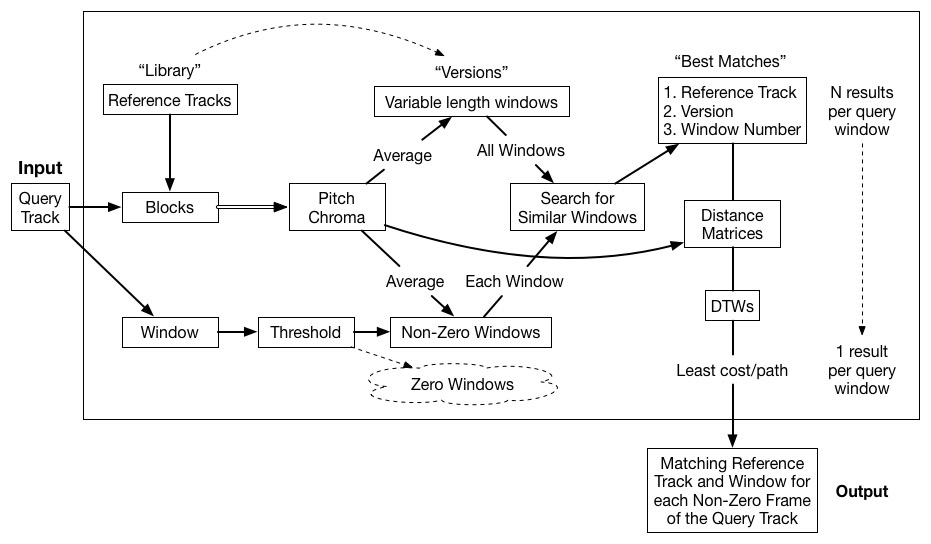
\includegraphics[width=\linewidth]{figs/APLSystem2.jpg}
\caption{A block diagram of the preliminary algorithm including the basic components of pause/silence removal, pitch chroma extraction, candidate identification, dynamic time warping, and reference estimation.}
\label{fig:APLSystem}
\end{figure}%

%Pitch chroma are computed from blocks of the query track, and averaged to fill frames that pass a threshold for amount of silence. These query frames of pitch chroma are used to search variable length frames of pitch chroma for each reference track. Dynamic time warping is applied to a collection of ``best matches'' for each query frame to choose the best result.

A block diagram of the algorithm is provided in Figure \ref{fig:APLSystem}. We begin with a library of ``reference tracks'' that are full-length recordings of the repertoire being practiced. These reference tracks can, for example, be a commercial CD recording or a full recording of the student or teacher's performance. After blocking these tracks, we compute a 12-dimensional pitch chroma vector per block. The pitch chroma captures the tonal content of the block mapped across the 12 note chromatic scale \cite{bartsch2001catch}. We aggregate multiple pitch chromas by averaging them over larger texture windows with pre-defined lengths. Windows containing silence are dropped. The results of this computation are then multiple chroma matrices for each of the reference tracks.

Incoming query tracks are processed similarly. For each query texture window, a distance to all reference windows is calculated in order to select the candidates with the least distance. Subsequently, we compute the DTW cost between the selected reference texture window and the query texture window using the original (not aggregated) pitch chroma blocks. The DTW cost is the overall cost of warping the subsequence pitch chroma matrix from the query texture window to the reference pitch chroma matrix \cite{Müller2007}. The reference track with the least DTW cost is chosen as the match for the query window.


\subsection{Feature Extraction}
\label{ref:FeatExt}

The pitch chroma is extracted in blocks of length 4096 samples with 50\% overlap, corresponding to approximately 93 ms. The pitch chromas are then averaged into texture windows of 16 times the block length, with 7/8 overlap between neighboring window for the query audio. As a preprocessing step, silences are ignored. Windows which contain more than 50\% samples with magnitude less than a threshold %of 0.02 
%{\color{red}{so the audio is normalized? No, the audio }} 
are dropped and labeled as zero windows. The remaining windows are labeled non-zero windows and are used for search.
%
The feature extraction for the reference tracks is identical, however, multiple texture window lengths are used in order to account for different possible tempi. More specifically, lengths ranging from $N=8, 10, 12, 14, 16, 18$ times the block size are used. Note that the length distribution is biased towards shorter windows as the query audio is more likely to be played slower than the reference.
%
At the end of this step, we have an aggregated pitch chroma vector for the query audio and a set of aggregated pitch-chroma matrices for the reference tracks. 

\subsection{Candidate Track Selection}
A match between query and reference is likely if the aggregated query pitch chroma matches one of the aggregated reference pitch chromas.
We select a group of 15 likely track candidates for each reference track by computing the Euclidean distance between the query vector and all reference track vectors.
% 
At the end of this step, we have a pool of 15 candidates across all window lengths across for each of the reference tracks, making 45 matches total.

\subsection{Track Identification}
\label{sec:DTW}
For the last step, we step back to the original short-time pitch chroma sequence. This means that our query track and reference tracks are now represented as a matrix of dimension $12\times (2N-1)$, where $N=16$ for the query track and $N=\{8,10,12,14,16,18\}$ for the reference tracks.
%
The DTW cost is then computed for all 45 pairs of query matrix and reference matrices. For all pairs, the reference track with the texture window that has the lowest DTW cost relative to its path length and reference window size 
%normalized by the path length {\color{red}{that is correct, isn't it?} Ouch, it may be correct, but not what we have done. We added a a scaling by window size that cancels out the original path length. This favors path-lengths that end early.}, 
is chosen as the repertoire piece being practiced in that particular texture window of the query audio.  Additional information such as the matching texture window length and matching frame are available, but not analyzed presently. 

Using this sequence of steps, texture windows in the reference library will be chosen for each query texture window. These windows correspond to particular locations in the reference tracks, while the window sizes correspond to the best matching tempo. 
%{\color{red}{the following sentence belongs to the next section, doesn't it?}} 
Figure~\ref{fig:140514-013} 
% Updated the plot.{\color{red}{I really think we need a proper plot showing proper results. This plot format is unhelpful and difficult to comprehend.}} 
presents the results of running this algorithm on all of the non-zero frames of one track of practiced audio. The majority of the windows identify as the correct track.

\begin{figure}
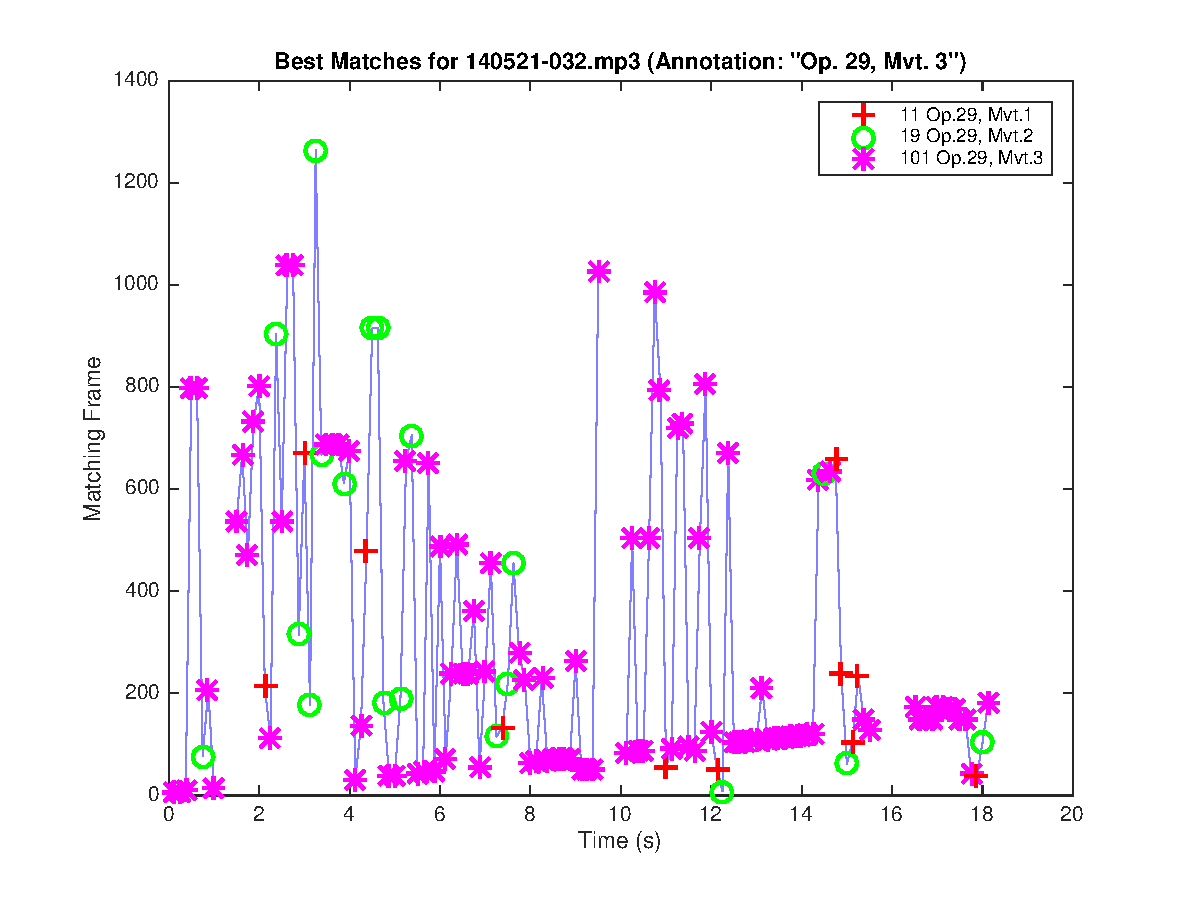
\includegraphics[width=\linewidth]{figs/minMatchingFrames.eps}
\caption{A figure displaying the algorithms identification of reference tracks and cost (dis-similarity) for all non-zero windows of a 67s query track of repertoire practice.}
\label{fig:140514-013}
\end{figure}

\subsection{Candidate Reduction}
\label{sec:reduction}
Before taking the DTW of all candidate windows, and choosing the one with the least weighted cost, there are a selection of 45 candidate locations---15 for each reference track. Before choosing the single best match for each query window, one can reduce the number of candidates using contextual information.  Specifically, a matching window $W_r$ in a reference track is more likely to be a correct match for a window in the query track $W_q$ if the following frame in the query track $W_{q+1}$ matches $W_r$ or $W_{r+1}$, and if the relative tempi are constant. Although this assumption will not hold for query frames followed by a large jump, pause, or with mistake, or decreasing tempo it can hold in many cases.

Leveraging this knowledge a function was written that eliminates candidate frames that did not meet the following three conditions:
\begin{itemize}
\item $W_{r+1} >= W_r$
\item $W_{r+1} <= W_r + 1$
\item Window length($W_r$) == Window length($W_{r+1}$)
\end{itemize}

These conditions can be applied recursively, eliminating more and more frames. This recursive process is demonstrated in Figure \ref{fig:reduction}.

\begin{figure}
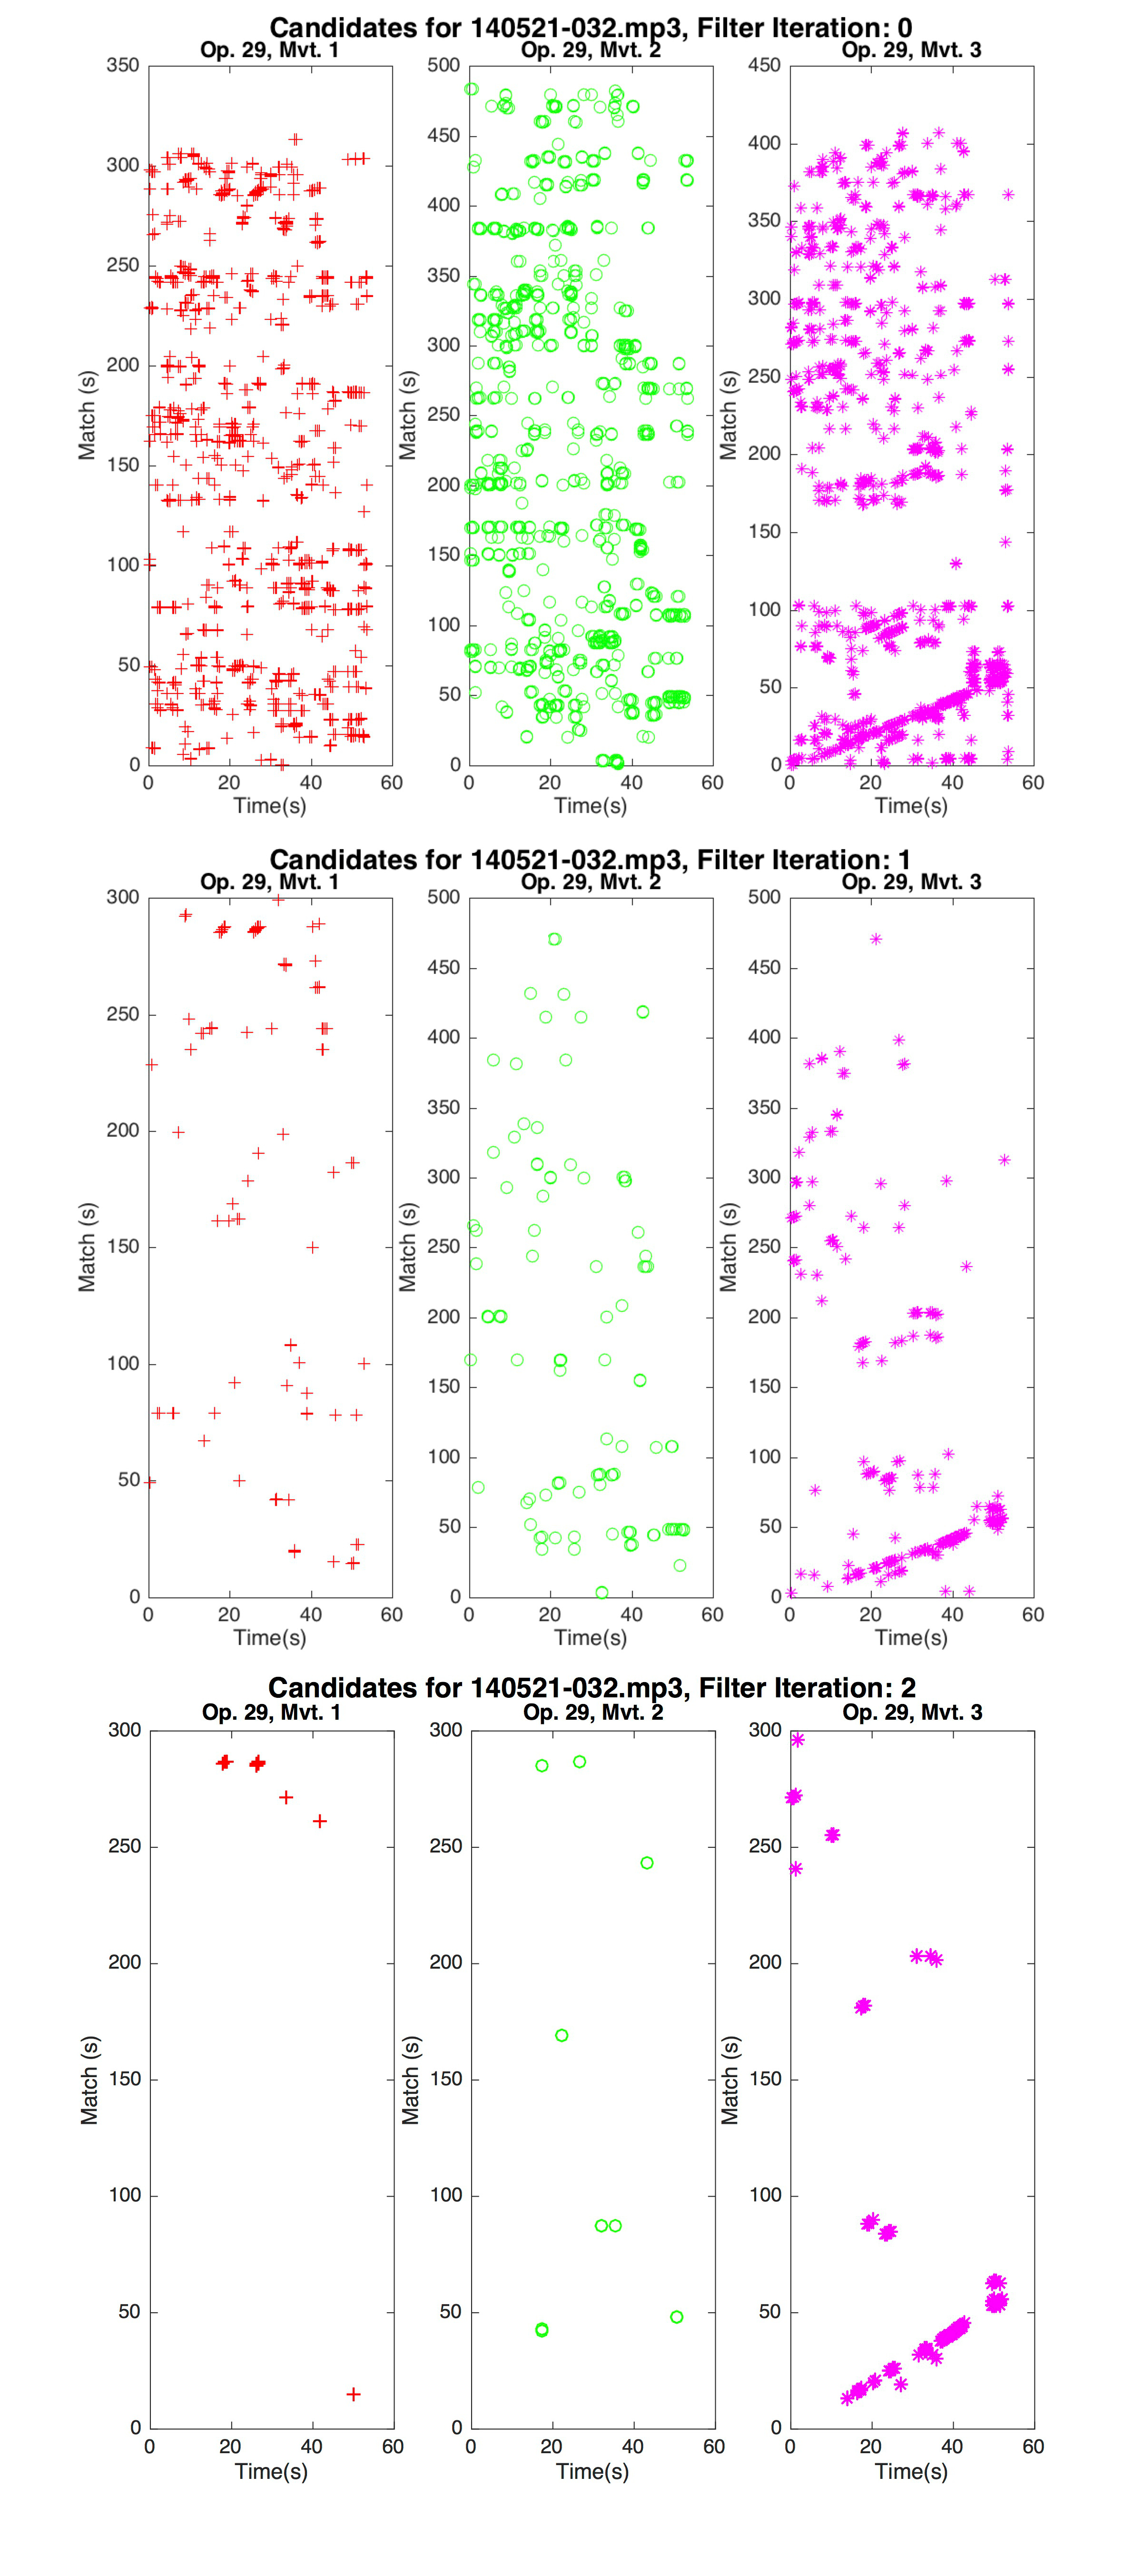
\includegraphics[width=\linewidth]{figs/Stepwise.jpg}
\caption{A figure displaying the results of candidate reduction. The three plots represent candidates in each of the three reference tracks for every frame of the query track. By iteratively applying the filter described in \ref{sec:reduction}, more and more candidates can be eliminated.}
\label{fig:reduction}
\end{figure}





\section{Results}
\label{sec:Results}

To test our approach on a large body of practice audio, we ran our algorithm on ~50,000 windows of practice from the APL dataset. As our approach is targeted towards repertoire practice, we chose recordings from a piece the performer was working towards at that time, namely Prokofiev's \textit{Piano Soanta No. 4 in C-Minor, Op. 29}. The piece is a three movement work including sections of various tempi, note-densities, tonal strengths and key centers, and at various levels of completion and familiarity.

To create a roughly even distribution of query windows across the three reference tracks, particular days in the APL dataset were chosen for analysis.  The APL dataset includes a disproportionate amount of work on the third movement, so days were selected that included relatively more work on the first and second movements. These were May 5th, 7th, 11th, 14th, 15th, 21st and 22nd.  Our analysis focused specifically on repertoire, so tracks annotated as `Technique,' `Sight Reading,' or `Improvisation' were not included. Furthermore, tracks that included annotations in the `Other' category were not included as this category was used to indicate tracks with audio sources not from the instrument (e.g. metronome, humming, singing, counting, but also distortion). Last, tracks that included more than one piece being practiced, or more than one kind of practice were not included.  A confusion matrix displaying the results of this test are displayed in Table \ref{tab:confMat}.  

%Table \ref{tab:confMat} displays a confusion matrix for the results. 

\begin{table}[ht!]
\centering
\caption{A confusion matrix for the 50,000 windows belonging to either Mvt. 1, 2 or 3.}
\begin{tabular}{|c|c|c|c|}
\hline
& \textbf{Mvt. 1} & \textbf{Mvt. 2} & \textbf{Mvt. 3} \\\hline
\textbf{Mvt. 1} & 0.55 & 0.29 & 0.15 \\\hline
\textbf{Mvt. 2} & 0.17 & 0.66 & 0.17 \\\hline
\textbf{Mvt. 3} & 0.13 & 0.21 & 0.66 \\\hline
\end{tabular}
\label{tab:confMat}
\end{table}

\section{Discussion}

The present results demonstrate that an APL system based upon the pitch chroma of short windows of practice audio can be used to identify the piece being practiced. The results target the broadest level of description, specifically the correct identification of the piece being practiced. However, further levels of detail are provided by this approach: namely a specific location in the reference track, the window size corresponding to the match, and the amount of dissimilarity (cost) for that combination. 
%Annotating window by window for this size of query (i.e. 50,000 windows) is not practical, in instead one might annotate based upon sections and subsections of a given piece.

Although the present results are far from perfect, it is important to remember that APL by nature identifies audio that is error-laden. Pauses, short-repetitions, wrong-notes and general fragmentation make correct identification of every window an unreasonable goal. Instead it is more practical for APL to use some form of interpolation. In the example of the present algorithm, a single window that is identified as Op. 29, Mvt. 2 that is surrounded by windows that are classified as belonging to a particular section in Op. 29, Mvt. 1, likely belongs to Mvt. 1. One could also interpolate by favoring windows in the reference tracks that are in a sequence, or are have the same window length (same relative tempo). It is interesting to note that for the present results, a simple majority vote for non-zero windows across each query track could be used to force windows from minority identifications to choose from windows in the majority identification. Even this course interpolation would lead to dramatic improvements in the confusion matrix of Table \ref{tab:confMat}. 

%into the ``proper'' identification, ostensibly providing 100\% identification accuracy. A better approach for the future would be to include an additional ``path-finding" step after the DTW, whereby the top 45 candidate windows and window sizes are kept for each query window. By assuming a loosely bounded continuity in tempo and linearity in time, likely ``paths" for window sequences can be computed. 

It is also necessary to acknowledge the importance of reference tracks in APL. In the present case, we make use of ``full versions'' of the repertoire pieces played by the same performer in a similar recording environment as the practiced audio. However, in general, complete versions of repertoire pieces are not available until the performer has already practiced them significantly.  Although one could choose to use studio recordings as reference, recording and production artifacts like microphone placement, SNR, spectral and temporal effects and reverberation may leave traces in the feature vector that can make correct identification more difficult. Furthermore, each performer and performance is subject to subtle timing deviations, which may create a systematic deviation when trying to match with those of the user. A better solution might be to use audio from a reference MIDI score, which would provide the highest amount of control and the additional benefit of measure numbers for matches. Generating ``reference'' material from the performer themselves however remains an interesting prospect for APL, which might have the most use when a score is not available (e.g. improvisation, new music).        






%As the length of an analysis window increases, the window is more likely to include a short repetition or large jump. Short repetitions are analogous to a stutter in speach, and occur when the performer is unsure of the note they are playing, or the following notes. Playing a small selection of notes in short

%such as to repeat a section (start from the beginning), or to move to another section altogether. As the analysis window decreases in size, it becomes less likely that the window will include a jump in the score, but there becomes less material on which to run an analysis.   

%Even a repetition of one note 



%However, an even finer level of segmentation is used for analysis. Our approach is to analyze large windows (1.5s to 3 seconds, or 16 - 32 window sizes) 


%As mentioned in the dataset description, silences longer than four seconds are discarded automatically. However, there are still many silences in the practiced audio that need to be handled with care.   

% \section{Future Work}

% \subsection{Algorithm}

% \begin{itemize}
% \item Onset-based windowing (i.e. have it start exactly on the onset).
% \end{itemize}

% \subsection{Annotations}

% \begin{itemize}
% \item More annotations
% \item Annotations of section being practiced
% \end{itemize}

\section{Conclusion}
This paper has presented current efforts towards Automatic Practice Logging (APL) including an annotated dataset, and a preliminary approach to identification.  Practice is a ubiquitous component of music, and despite challenges, there are many benefits to logging its content automatically. Practice occurs in many forms, and for the purpose of annotating it, we presented a typology and annotation framework that can be generalized to many instruments, musicians and types of practice.  We presented a proof of concept algorithm that that searches a reference library using pitch-chroma computed on very short segments, and using dynamic-time warping as an additional step to find the best match from a collection of candidates. Incorporating additional local assumptions such as score-continuity and constant tempo might lead to increased performance in the future, but one should be mindful that practice is globally fragmented and variable in tempo. Together, we hope that this work will encourage others to explore APL as an interesting and valuable topic for MIR.     

% For bibtex users:
\bibliography{ISMIRtemplate}

% For non bibtex users:
%\begin{thebibliography}{citations}
%
%\bibitem {Author:00}
%E. Author.
%``The Title of the Conference Paper,''
%{\it Proceedings of the International Symposium
%on Music Information Retrieval}, pp.~000--111, 2000.
%
%\bibitem{Someone:10}
%A. Someone, B. Someone, and C. Someone.
%``The Title of the Journal Paper,''
%{\it Journal of New Music Research},
%Vol.~A, No.~B, pp.~111--222, 2010.
%
%\bibitem{Someone:04} X. Someone and Y. Someone. {\it Title of the Book},
%    Editorial Acme, Porto, 2012.
%
%\end{thebibliography}

\end{document}
